\chapter{Implementation and Performance Analysis}
In the previous section, we described the system's general architecture and the modules required to implement the tracking system. In this chapter, we will explain how the different parts are connected, and we will explain the implementation of the system.\\
The tracking system designed in this project uses Arduino module and the ُSIM 808, including the GSM and GPS antennas, for tracking. The core of this project is the Arduino microcontroller. The geographical location of object is received using a GPS antenna, and then this information is sent to the webserver using GSM technology. A web application has been developed to view and track an object on a map. This application consists of two parts: Front-end and Back-end. The front-end part has developed using Angular framework, and the Back-end part has developed using Express framework.\\
Initially, the SIM 808 module is initialized to get the location from the satellite. The initial settings of this device are done using AT commands. By connecting the GPS antenna, this module will be able to receive location coordinates from the satellite. Then the settings related to the GPRS network are done.\\
In fiqure 3.1 How to connect different modules in the tracking system is shown:\\
\begin{figure}[!h]
	\centerline{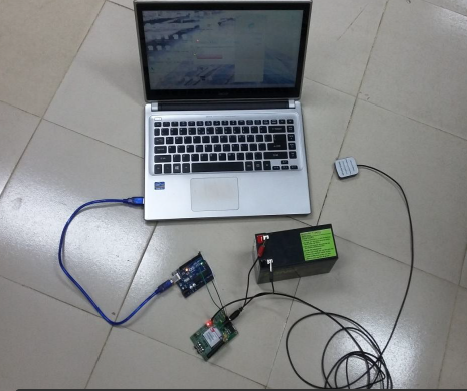
\includegraphics[width=.7\textwidth]{design-system}}
	\caption{Designed Tracking System}
\end{figure}\\
\section{Evaluate Tracking system performance}
As mentioned, the hardware part of our system consists of four modules, SIM 808, GSM receiver, GPS receiver, and Arduino microcontroller. This section will explain the implementation of the designed system, how to connect the various components and the implemented code.
\subsection{Circuit performance evaluation}
Before dealing with the modules and how to connect them, it is necessary to observe the system microcontroller performance and processing information in the flowchart. The overall performance of the system was described in the previous section. Now we have a flowchart about the implemented algorithm, and we can have a better understanding of the workflow in the hardware circuit designed and the code written for it.\\
The following diagram shows the general process of the implemented code on the Arduino.
\begin{figure}[h!]
	\centering
	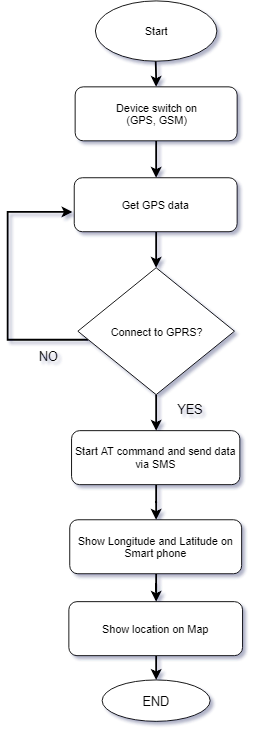
\includegraphics[width=.4\textwidth]{tracking-flowchart}
	\caption{Performance of implemented code on Arduino \cite{3}}
\end{figure}
\newpage
Firstly, for testing the system, the GPS antenna is connected to the SIM 808 module to receive the object's location (latitude and longitude) from the satellite. For doing this, the Arduino IDE software is used to program the code written on the Arduino board.\\
\newpage
The flowchart 3.3 shows how GPS works:\\
\begin{figure}[!h]
	\centerline{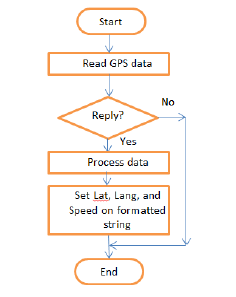
\includegraphics[width=.6\textwidth]{gps-flowchart}}
	\caption{Read Information diagram \cite{8}}
\end{figure}

For sending the object's location to the user via the GSM network, SIM 808 module and the Arduino microcontroller connected to it are used. For connecting 808 SIM module to the GSM network, we use AT commands to program and control it.\\
\newpage
The flowchart 3.4 shows how GSM works:\\
\begin{figure}[!h]
	\centerline{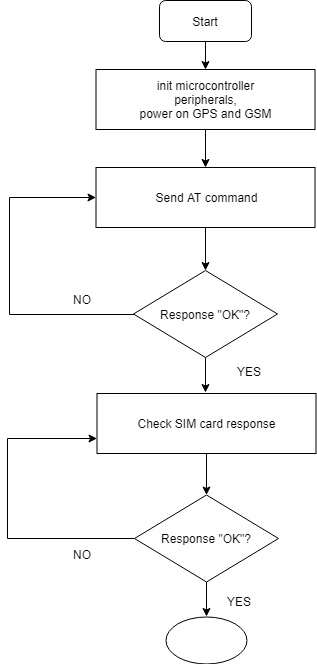
\includegraphics[width=.6\textwidth]{gsm-flowchart}}
	\caption{GSM \cite{8}}
\end{figure}
\newpage
\begin{figure}[!h]
	\centerline{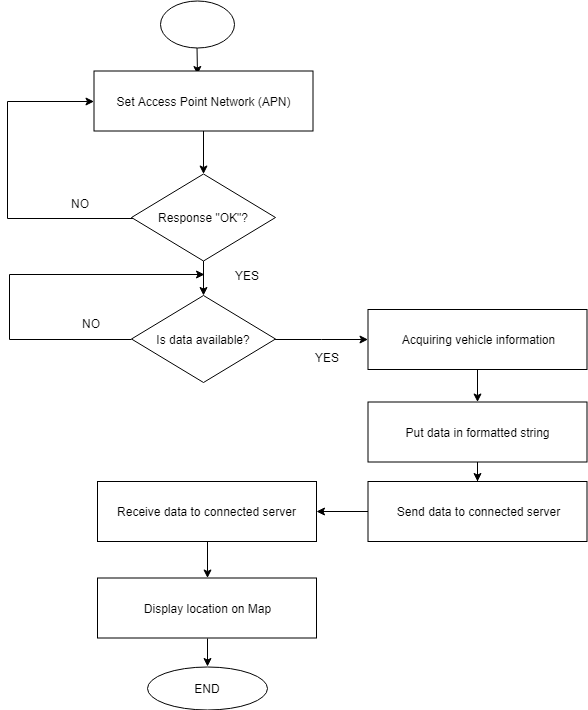
\includegraphics[width=.9\textwidth]{continue-gsm}}
	\caption{GSM \cite{8}}
\end{figure}